% Options for packages loaded elsewhere
\PassOptionsToPackage{unicode}{hyperref}
\PassOptionsToPackage{hyphens}{url}
%
\documentclass[
  ignorenonframetext,
  serif,
  professionalfont,
  usenames,
  dvipsnames,
  aspectratio = 169]{beamer}
\usepackage{pgfpages}
\setbeamertemplate{caption}[numbered]
\setbeamertemplate{caption label separator}{: }
\setbeamercolor{caption name}{fg=normal text.fg}
\beamertemplatenavigationsymbolsempty
% Prevent slide breaks in the middle of a paragraph
\widowpenalties 1 10000
\raggedbottom
\setbeamertemplate{part page}{
  \centering
  \begin{beamercolorbox}[sep=16pt,center]{part title}
    \usebeamerfont{part title}\insertpart\par
  \end{beamercolorbox}
}
\setbeamertemplate{section page}{
  \centering
  \begin{beamercolorbox}[sep=12pt,center]{part title}
    \usebeamerfont{section title}\insertsection\par
  \end{beamercolorbox}
}
\setbeamertemplate{subsection page}{
  \centering
  \begin{beamercolorbox}[sep=8pt,center]{part title}
    \usebeamerfont{subsection title}\insertsubsection\par
  \end{beamercolorbox}
}
\AtBeginPart{
  \frame{\partpage}
}
\AtBeginSection{
  \ifbibliography
  \else
    \frame{\sectionpage}
  \fi
}
\AtBeginSubsection{
  \frame{\subsectionpage}
}
\usepackage{amsmath,amssymb}
\usepackage{lmodern}
\usepackage{iftex}
\ifPDFTeX
  \usepackage[T1]{fontenc}
  \usepackage[utf8]{inputenc}
  \usepackage{textcomp} % provide euro and other symbols
\else % if luatex or xetex
  \usepackage{unicode-math}
  \defaultfontfeatures{Scale=MatchLowercase}
  \defaultfontfeatures[\rmfamily]{Ligatures=TeX,Scale=1}
\fi
% Use upquote if available, for straight quotes in verbatim environments
\IfFileExists{upquote.sty}{\usepackage{upquote}}{}
\IfFileExists{microtype.sty}{% use microtype if available
  \usepackage[]{microtype}
  \UseMicrotypeSet[protrusion]{basicmath} % disable protrusion for tt fonts
}{}
\makeatletter
\@ifundefined{KOMAClassName}{% if non-KOMA class
  \IfFileExists{parskip.sty}{%
    \usepackage{parskip}
  }{% else
    \setlength{\parindent}{0pt}
    \setlength{\parskip}{6pt plus 2pt minus 1pt}}
}{% if KOMA class
  \KOMAoptions{parskip=half}}
\makeatother
\usepackage{xcolor}
\newif\ifbibliography
\usepackage{longtable,booktabs,array}
\usepackage{calc} % for calculating minipage widths
\usepackage{caption}
% Make caption package work with longtable
\makeatletter
\def\fnum@table{\tablename~\thetable}
\makeatother
\usepackage{graphicx}
\makeatletter
\def\maxwidth{\ifdim\Gin@nat@width>\linewidth\linewidth\else\Gin@nat@width\fi}
\def\maxheight{\ifdim\Gin@nat@height>\textheight\textheight\else\Gin@nat@height\fi}
\makeatother
% Scale images if necessary, so that they will not overflow the page
% margins by default, and it is still possible to overwrite the defaults
% using explicit options in \includegraphics[width, height, ...]{}
\setkeys{Gin}{width=\maxwidth,height=\maxheight,keepaspectratio}
% Set default figure placement to htbp
\makeatletter
\def\fps@figure{htbp}
\makeatother
\setlength{\emergencystretch}{3em} % prevent overfull lines
\providecommand{\tightlist}{%
  \setlength{\itemsep}{0pt}\setlength{\parskip}{0pt}}
\setcounter{secnumdepth}{-\maxdimen} % remove section numbering
% Definição do esquema de cores:
% 1. UFPR - Azul com cinza.
% 2. DEST - Roxo com cinza.
% 3. LEG - Laranjado com cinza.
\def\mycolorscheme{1}

% Caminho para a imagem de fundo com aspecto 16x9.
% \def\pathtobg{config/ufpr-fachada-baixo-1.jpg}
% \def\pathtobg{config/ufpr-fundo.jpg}
% \def\pathtobg{config/ufpr-fundo.jpg}
\def\pathtobg{./config/ufpr-fundo-16x9.jpg}

% \providecommand{\tightlist}{%
%   \setlength{\itemsep}{0pt}\setlength{\parskip}{0pt}}
% ATTENTION: Redefine o comando acima que é definido pelo template.
% \renewcommand{\tightlist}{}
\renewcommand{\tightlist}{%
  \setlength{\itemsep}{0\baselineskip}
  \setlength{\parskip}{0.25\baselineskip}
}

% Logo na capa.
\titlegraphic{
  %\vspace{-1em}
  %\includegraphics[height=1.2cm]{config/dest-texto-2.png}\hspace{1em}
  %\includegraphics[height=1.8cm]{config/dsbd-logo-2x2.png}\hspace{1em}
  
\includegraphics[height=1.8cm]{config/ufpr-transparent-600px.png}
}
%-----------------------------------------------------------------------

% Palladio.
% \usepackage[sc]{mathpazo}
% \linespread{1.05}         % Palladio needs more leading (space between lines)
% \usepackage[T1]{fontenc}

% Kurier.
% \usepackage[light, condensed, math]{kurier}
% \usepackage[T1]{fontenc}

% Iwona.
% \usepackage[math, light, condensed]{iwona}

% \usepackage{cmbright}
% \usepackage[charter]{mathdesign}
% \usepackage{palatino}

% Roboto (with Iwona for maths).
% \usepackage[math]{iwona}
% \usepackage[sfdefault, light, condensed]{roboto}

% Source Sans Pro (with Iwona for maths).
% \usepackage[math]{iwona}
% \usepackage[default, light]{sourcesanspro}

% Lato (with Iwona for maths).
% \usepackage[math]{iwona}
% \usepackage[default]{lato}

% Fira Sans (with Iwona for maths).
\usepackage[math, light]{iwona}
\usepackage[sfdefault,light]{FiraSans} %% option 'sfdefault' activates Fira Sans as the default text font
\usepackage[T1]{fontenc}
\renewcommand*\oldstylenums[1]{{\firaoldstyle #1}}

% Font for code. ----------------------------
% \usepackage[scaled=.75]{beramono}
\usepackage{inconsolata}

% ATTENTION: needs complile with xelatex: `$ xelatex file.tex`
% \usepackage{fontspec}
% \setmonofont{M+ 1m}
% \setmonofont{M+ 1mn}
% \setmonofont{M+ 2m}

%-----------------------------------------------------------------------

% \usepackage{lmodern}
\usepackage{amssymb, amsmath}
\usepackage[makeroom]{cancel}
% \usepackage{ifxetex, ifluatex}
\usepackage{fixltx2e} % provides \textsubscript
\usepackage[utf8]{inputenc}
\usepackage[shorthands=off,main=brazil]{babel}
\usepackage{graphicx}
\usepackage{xcolor}
\usepackage{setspace}
\usepackage{comment}
\usepackage{icomma}

%-----------------------------------------------------------------------
% Algumas configurações.

\setlength{\parindent}{0pt}
\setlength{\parskip}{6pt plus 2pt minus 1pt}
\setlength{\emergencystretch}{3em}  % prevent overfull lines
% \providecommand{\tightlist}{%
%   \setlength{\itemsep}{0pt}\setlength{\parskip}{0pt}}
\setcounter{secnumdepth}{0}

% Espaço vertical para o ambiente `quote`.
\let\oldquote\quote
\let\oldendquote\endquote
\renewenvironment{quote}{%
  \vspace{1em}\oldquote}{%
  \oldendquote\vspace{1em}}

%-----------------------------------------------------------------------
% Espaçamento entre items para itemize, enumerate e description.

% % itemize.
% \let\itemopen\itemize
% \let\itemclose\enditemize
% \renewenvironment{itemize}{%
%   \itemopen\addtolength{\itemsep}{0.25\baselineskip}}{\itemclose}
%
% % enumerate.
% \let\enumopen\enumerate
% \let\enumclose\endenumerate
% \renewenvironment{enumerate}{%
%   \enumopen\addtolength{\itemsep}{0.25\baselineskip}}{\enumclose}
%
% % description.
% \let\descopen\description
% \let\descclose\enddescription
% \renewenvironment{description}{%
%   \descopen\addtolength{\itemsep}{0.25\baselineskip}}{\descclose}

%-----------------------------------------------------------------------

% \usepackage[hang]{caption}
\usepackage{caption}
\captionsetup{font=footnotesize,
  labelfont={color=mycolor1, footnotesize},
  labelsep=period}

% \providecommand{\tightlist}{%
%   \setlength{\itemsep}{0pt}\setlength{\parskip}{0pt}}

%-----------------------------------------------------------------------

\usepackage{tikz}

% \def\pathtobg{/home/walmes/Projects/templates/COMMON/ufpr-fundo.jpg}
% \def\pathtobg{/home/walmes/Projects/templates/COMMON/ufpr-fundo-16x9.jpg}
% \def\pathtobg{/home/walmes/Projects/templates/COMMON/ufpr-fachada-dir-1.jpg}
% \def\pathtobg{/home/walmes/Projects/templates/COMMON/ufpr-fachada-esq-1.jpg}
% \def\pathtobg{/home/walmes/Projects/templates/COMMON/ufpr-perto-1.jpg}
% \def\pathtobg{/home/walmes/Projects/templates/COMMON/ufpr-fachada-baixo-1.jpg}

\ifx\pathtobg\undefined
\else
  \usebackgroundtemplate{
    \tikz[overlay, remember picture]
    \node[% opacity=0.3,
          at=(current page.south east),
          anchor=south east,
          inner sep=0pt] {
            \includegraphics[height=\paperheight, width=\paperwidth]{\pathtobg}};
  }
\fi

%-----------------------------------------------------------------------
% Definições de esquema de cores.

\ifx\mycolorscheme\undefined
  % UFPR.
  % http://www.color-hex.com/color-palette/2018
  \definecolor{mycolor1}{HTML}{015c93} % Título.
  \definecolor{mycolor2}{HTML}{363435} % Texto.
  \definecolor{mycolor3}{HTML}{015c93} % Estrutura.
  \definecolor{mycolor4}{HTML}{015c93} % Links.
  \definecolor{mycolor5}{HTML}{CECAC5} % Preenchimentos.
\else
  \if\mycolorscheme1
    % UFPR.
    \definecolor{mycolor1}{HTML}{015c93} % Título.
    \definecolor{mycolor2}{HTML}{363435} % Texto.
    \definecolor{mycolor3}{HTML}{015c93} % Estrutura.
    \definecolor{mycolor4}{HTML}{015c93} % Links.
    \definecolor{mycolor5}{HTML}{CECAC5} % Preenchimentos.
  \fi
  \if\mycolorscheme2
    % DEST.
    \definecolor{mycolor1}{HTML}{2a0e72} % Título.
    \definecolor{mycolor2}{HTML}{202E35} % Texto.
    \definecolor{mycolor3}{HTML}{2a0e72} % Estrutura.
    % \definecolor{mycolor3}{HTML}{8072a3} % Estrutura.
    \definecolor{mycolor4}{HTML}{2a0e72} % Links.
    % \definecolor{mycolor4}{HTML}{bfb9d1} % Links.
    % \definecolor{mycolor5}{HTML}{AEA79F} % Preenchimentos.
    \definecolor{mycolor5}{HTML}{CECAC5} % Preenchimentos.
  \fi
  \if\mycolorscheme3
    % LEG.
    \definecolor{mycolor2}{HTML}{363435} % Texto.
    % \definecolor{mycolor1}{HTML}{ff8000} % Título.
    % \definecolor{mycolor3}{HTML}{ff8000} % Estrutura.
    % \definecolor{mycolor4}{HTML}{ff8000} % Links.
    % \definecolor{mycolor1}{HTML}{E57300} % Título.
    % \definecolor{mycolor3}{HTML}{E57300} % Estrutura.
    % \definecolor{mycolor4}{HTML}{E57300} % Links.
    \definecolor{mycolor1}{HTML}{F67014} % Título.
    \definecolor{mycolor3}{HTML}{F67014} % Estrutura.
    \definecolor{mycolor4}{HTML}{F67014} % Links.
    % \definecolor{mycolor1}{HTML}{FE5C23} % Título.
    % \definecolor{mycolor3}{HTML}{FE5C23} % Estrutura.
    % \definecolor{mycolor4}{HTML}{FE5C23} % Links.
    \definecolor{mycolor5}{HTML}{222222} % Preenchimentos.
    \definecolor{mycolor5}{HTML}{383838} % Preenchimentos.
  \fi
\fi

\hypersetup{
  colorlinks=true,
  linkcolor=mycolor4,
  urlcolor=mycolor1,
  citecolor=mycolor1
}

%-----------------------------------------------------------------------
% ATTENTION: http://www.cpt.univ-mrs.fr/~masson/latex/Beamer-appearance-cheat-sheet.pdf

\usetheme{Boadilla}
\usecolortheme{default}

% \setbeamersize{text margin left=7mm, text margin right=7mm}
% \setbeamertemplate{frametitle}[default][left, leftskip=3mm]
% \addtobeamertemplate{frametitle}{\vspace{0.5em}}{}

\setbeamertemplate{caption}[numbered]
\setbeamertemplate{section in toc}[sections numbered]
\setbeamertemplate{subsection in toc}[subsections numbered]
\setbeamertemplate{sections/subsections in toc}[ball]{}
\setbeamertemplate{sections in toc}[ball]
\setbeamercolor{section number projected}{bg=mycolor1, fg=white}
\setbeamertemplate{blocks}[rounded]
\setbeamertemplate{navigation symbols}{}
\setbeamertemplate{frametitle continuation}{\gdef\beamer@frametitle{}}
% \setbeamertemplate{frametitle}[default][center]
% \setbeamertemplate{footline}[frame number]

\setbeamertemplate{enumerate items}[default]
\setbeamertemplate{itemize items}{\scriptsize\raise1.25pt\hbox{\donotcoloroutermaths$\blacktriangleright$}}

% Blocos.
% \addtobeamertemplate{block begin}{\vskip -\bigskipamount}{}
% \addtobeamertemplate{block end}{}{\vskip -\bigskipamount}
\addtobeamertemplate{block begin}{\vspace{0.5em}}{}
\addtobeamertemplate{block end}{}{\vspace{0.5em}}


% Rodapé.
\setbeamercolor{title in head/foot}{parent=subsection in head/foot}
\setbeamercolor{author in head/foot}{bg=mycolor4, fg=white}
\setbeamercolor{date in head/foot}{parent=subsection in head/foot, fg=mycolor3}

% Cabeçalho.
\setbeamercolor{section in head/foot}{bg=mycolor2, fg=mycolor4}
\setbeamercolor{subsection in head/foot}{bg=mycolor2, fg=white}

\setbeamercolor{title}{fg=mycolor1}       % Título dos slides.
\setbeamercolor{titlelike}{fg=title}
\setbeamercolor{subtitle}{fg=mycolor2}    % Subtítulo.
\setbeamercolor{institute in head/foot}{parent=palette primary} % Instituição.
\setbeamercolor{frametitle}{fg=mycolor1}  % De quadro.
\setbeamercolor{structure}{fg=mycolor3}   % Listas e rodapé.
\setbeamercolor{item projected}{bg=mycolor2}
\setbeamercolor{block title}{bg=mycolor5, fg=mycolor2}
\setbeamercolor{normal text}{fg=mycolor2} % Texto.
\setbeamercolor{caption name}{fg=normal text.fg}
% \setbeamercolor{footlinecolor}{fg=mycolor2, bg=mycolor5}
% \setbeamercolor{section in head/foot}{fg=mycolor2, bg=mycolor5}
\setbeamercolor{author in head/foot}{fg=white, bg=mycolor1}
\setbeamercolor{section in foot}{fg=mycolor4, bg=mycolor5}
\setbeamercolor{date in foot}{fg=mycolor4, bg=mycolor5}
\setbeamercolor{block title}{fg=white, bg=mycolor1}
\setbeamercolor{block body}{fg=black, bg=white!80!gray}
\setbeamercolor{block body}{fg=black, bg=white!80!gray}

% To remove empty brackets of \institution.
\makeatletter
\setbeamertemplate{footline}{
  \leavevmode%
  \hbox{%
    \begin{beamercolorbox}[
      wd=0.3\paperwidth, ht=2.25ex, dp=1ex, right]{author in head/foot}%
      \usebeamerfont{author in head/foot}\insertshortauthor{}\hspace*{1ex}
    \end{beamercolorbox}%
    \begin{beamercolorbox}[
      wd=0.6\paperwidth, ht=2.25ex, dp=1ex, left]{section in foot}%
      \usebeamerfont{title in head/foot}\hspace*{1ex}\insertshorttitle{}
      % \usebeamerfont{title in head/foot}\hspace*{1ex}\insertframetitle{}
    \end{beamercolorbox}%
    \begin{beamercolorbox}[
      wd=0.1\paperwidth, ht=2.25ex, dp=1ex, right]{date in foot}%
      \insertframenumber{}\hspace*{2ex}
    \end{beamercolorbox}
  }%
  \vskip0pt%
}
\makeatother

%-----------------------------------------------------------------------

% \usepackage{hyphenat}
\usepackage{changepage}

% Slide para o título das seções.
\AtBeginSection[]{
  \begin{frame}
    % \vfill
    \vspace{4cm}
    % \centering
    % \begin{beamercolorbox}[sep = 8pt, center, shadow = true, rounded = true]{title}
    \begin{beamercolorbox}{title}
      \begin{columns}
        \column{0.7\linewidth}
        {\LARGE\textbf \insertsectionhead}
      \end{columns}
    \end{beamercolorbox}
    \vfill
  \end{frame}
}

%-----------------------------------------------------------------------
%---- preamble-chunk.tex -----------------------------------------------

% Knitr.

% ATTENTION: this needs `\usepackage{xcolor}'.
\definecolor{color_line}{HTML}{333333}
\definecolor{color_back}{HTML}{DDDDDD}
% \definecolor{color_back}{HTML}{FF0000}

% ATTENTION: usa o fancyvrb.
% https://ctan.math.illinois.edu/macros/latex/contrib/fancyvrb/doc/fancyvrb-doc.pdf
% R input.
\usepackage{tcolorbox}
\ifcsmacro{Highlighting}{
  % Statment if it exists. ------------------
  \DefineVerbatimEnvironment{Highlighting}{Verbatim}{
    % frame=lines,     % Linha superior e inferior.
    % framerule=0.5pt, % Espessura da linha.
    framesep=2ex,    % Distância da linha para o texto.
    % rulecolor=\color{color_line},
    % numbers=right,
    fontsize=\footnotesize, % Tamanho da fonte.
    baselinestretch=0.8,    % Espaçamento entre linhas.
    commandchars=\\\{\}}
  % Margens do ambiente `Shaded'.
  % \fvset{listparameters={\setlength{\topsep}{-1em}}}
  % \renewenvironment{Shaded}{\vspace{-1ex}}{\vspace{-2ex}}
  \renewenvironment{Shaded}{
    \vspace{2pt}
    \begin{tcolorbox}[
      boxrule=0pt,      % Espessura do contorno.
      colframe=gray!10, % Cor do contorno.
      colback=gray!10,  % Cor de fundo da caixa.
      arc=1em,          % Raio para contornos arredondados.
      sharp corners,
      boxsep=0.5em,     % Margem interna.
      left=3pt, right=3pt, top=3pt, bottom=3pt, % Margens internas.
      grow to left by=0mm,
      grow to right by=6pt,
      ]
    }{
    \end{tcolorbox}
    \vspace{-3pt}
    }
  }{
  % Statment if it not exists. --------------
}

% R output e todo `verbatim'.
\makeatletter
\def\verbatim@font{\linespread{0.8}\ttfamily\footnotesize}
%\makeatother

% Cor de fundo e margens do `verbatim'.
\let\oldv\verbatim
\let\oldendv\endverbatim

\def\verbatim{%
  \par\setbox0\vbox\bgroup % Abre grupo.
  %\vspace{-5px}            % Reduz margem superior.
  \oldv                    % Chama abertura do verbatim.
}
\def\endverbatim{%
  \oldendv                 % Chama encerramento do verbatim.
  %\vspace{0cm}           % Controla margem inferior.
  \egroup%\fboxsep5px      % Fecha grupo.
  \noindent{{\usebox0}}\par
}

%-----------------------------------------------------------------------
%---- preamble-commands.tex --------------------------------------------

% Para fazer texto em duas colunas.
\newcommand{\mytwocolumns}[4]{
  % #1: Line width fraction for the left column , e.g. 0.5.
  % #2: Line width fraction for the right column.
  % #3: Content for the left column.
  % #4: Content for the right column.
  \begin{columns}[c]
    \begin{column}{#1\linewidth} %----------- left.
      #3
    \end{column} %--------------------------- left.
    \begin{column}{#2\linewidth} %----------- right.
      #4
    \end{column} %--------------------------- right.
  \end{columns}
}

%-----------------------------------------------------------------------
% Para fazer duas colunas no Rmd.

% Center vertical align.
\def\beginAHalfColumn{\begin{minipage}{0.49\textwidth}}%
\def\beginAlmostHalfColumn{\begin{minipage}{0.45\textwidth}}%
\def\beginAQuarterColumn{\begin{minipage}{0.23\textwidth}}%
\def\beginThreeQuartersColumn{\begin{minipage}{0.72\textwidth}}%
\def\beginAThirdColumn{\begin{minipage}{0.31\textwidth}}%
\def\beginTwoThirdsColumn{\begin{minipage}{0.64\textwidth}}%
\def\endColumns{\end{minipage}}%

% Top vertical align.
\def\beginAHalfColumnT{\begin{minipage}[t]{0.49\textwidth}}%
\def\beginAlmostHalfColumnT{\begin{minipage}[t]{0.45\textwidth}}%
\def\beginAQuarterColumnT{\begin{minipage}[t]{0.23\textwidth}}%
\def\beginThreeQuartersColumnT{\begin{minipage}[t]{0.72\textwidth}}%
\def\beginAThirdColumnT{\begin{minipage}[t]{0.31\textwidth}}%
\def\beginTwoThirdsColumnT{\begin{minipage}[t]{0.64\textwidth}}%

%---------------------------------------------------------------------
% Ambientes para frases como e sem imagem.

\newcommand{\myquote}[3]{
  % #1: caminho para a imagem.
  % #2: a frase/quotation.
  % #3: o autor.
  \begin{center}
    \begin{minipage}[c]{0.19\linewidth}
      \begin{center}
        \includegraphics[height=2.5cm]{#1}
      \end{center}
    \end{minipage}
    \begin{minipage}[c]{0.7\linewidth}
      \begin{flushright}
        \textit{#2}
        \vspace{1ex}

        -- #3
      \end{flushright}
    \end{minipage}
  \end{center}
}

\newcommand{\myphrase}[2]{
  % #1: a frase/quotation.
  % #2: o autor.
  \begin{center}
    \begin{minipage}[c]{0.19\linewidth}
    \end{minipage}
    \begin{minipage}[c]{0.7\linewidth}
      \begin{flushright}
        \textit{#1}
        \vspace{1ex}

        -- #2
      \end{flushright}
    \end{minipage}
  \end{center}
}

%-----------------------------------------------------------------------
% Comandos para texto em destaque.

% \newcommand{\hi}[1]{%
%   \textcolor{ubuntu_orange}{#1}\xspace
% }

\usepackage{xspace}

% URLs com letra miuda.
\newcommand{\myurl}[1]{%
  {\tiny \url{#1}}\xspace
}

% Botões.
\newcommand{\btn}[1]{%
  \beamergotobutton{#1}\xspace
}

% Texto grande centralizado.
\newcommand{\centertitle}[1]{%
  \begin{center}
    {\LARGE \bfseries \hi{#1}}
  \end{center}
}

%-----------------------------------------------------------------------
\ifLuaTeX
  \usepackage{selnolig}  % disable illegal ligatures
\fi
\IfFileExists{bookmark.sty}{\usepackage{bookmark}}{\usepackage{hyperref}}
\IfFileExists{xurl.sty}{\usepackage{xurl}}{} % add URL line breaks if available
\urlstyle{same} % disable monospaced font for URLs
\hypersetup{
  pdfauthor={Prof.~Me. Lineu Alberto Cavazani de Freitas},
  hidelinks,
  pdfcreator={LaTeX via pandoc}}

\title{\textbf{Análise exploratória II}}
\subtitle{Resumos numéricos - medidas de posição e dispersão.}
\author{Prof.~Me. Lineu Alberto Cavazani de Freitas}
\date{}
\institute{\textbf{CE003 – Estatística II}\\
\strut \\
Departamento de Estatística\\
Laboratório de Estatística e Geoinformação}

\begin{document}
\frame{\titlepage}

\begin{frame}{Resumos numéricos}
\protect\hypertarget{resumos-numuxe9ricos}{}
\begin{itemize}
\item
  Uma forma de resumir a informação contida em um conjunto de dados é
  por meio dos \textbf{resumos numéricos}.
\item
  Resumos numéricos são basicamente
  \textbf{números que resumem números}.
\item
  Os dois principais grupos são as medidas de \textbf{posição} (central
  e relativa) e \textbf{dispersão}.
\item
  Existem outros conjuntos de medidas, como as medidas de \textbf{forma}
  e também as de \textbf{relação/associação}.
\end{itemize}
\end{frame}

\hypertarget{medidas-de-posiuxe7uxe3o-central}{%
\section{Medidas de posição
central}\label{medidas-de-posiuxe7uxe3o-central}}

\begin{frame}{Medidas de posição central}
\protect\hypertarget{medidas-de-posiuxe7uxe3o-central-1}{}
\beginAHalfColumn

\begin{itemize}
\tightlist
\item
  As medidas de posição central buscam expressar o \textbf{centro} de
  uma variável por meio de ideias como:

  \begin{itemize}
  \tightlist
  \item
    Centro de massa.
  \item
    Valor que divide a amostra em partes iguais.
  \item
    Valores de maior frequência ou densidade.
  \end{itemize}
\end{itemize}

\endColumns
\beginAHalfColumn

\begin{itemize}
\tightlist
\item
  Algumas possiblidades são

  \begin{itemize}
  \tightlist
  \item
    Média.
  \item
    Mediana.
  \item
    Moda.
  \item
    Média geométrica.
  \item
    Média harmônica.
  \item
    Média aparada.
  \end{itemize}
\end{itemize}

\endColumns
\end{frame}

\begin{frame}{Média aritmética}
\protect\hypertarget{muxe9dia-aritmuxe9tica}{}
\begin{itemize}
\tightlist
\item
  Soma de todos os valores dividida pela quantidade de elementos.
\item
  Interpretação física de centro de gravidade.
\item
  Medida influenciada por valores extremos.
\end{itemize}

\textbf{Expressão}

\[
      \overline{y} = \dfrac{\sum_{i = 1}^{n} y_i}{n} = \frac{y_1 + y_2 + \cdots + y_n}{n}.
\]
\end{frame}

\begin{frame}{Média aritmética}
\protect\hypertarget{muxe9dia-aritmuxe9tica-1}{}
\textbf{Exemplo}

\begin{itemize}
\item
  Considere que uma turma possui 10 alunos.
\item
  Estes alunos realizaram uma avaliação.
\item
  Considere que as notas obtidas foram:
\end{itemize}

\[60;\ 65;\ 77;\ 95;\ 56;\ 94;\ 97;\ 81;\ 80;\ 48\]

\begin{itemize}
\tightlist
\item
  Qual foi a nota média da turma?
\end{itemize}

\[
\overline{y}  = \frac{60+65+77+95+56+94+97+81+80+48}{10} = \frac{753}{10} = 75,3
\]
\end{frame}

\begin{frame}{Média aritmética ponderada}
\protect\hypertarget{muxe9dia-aritmuxe9tica-ponderada}{}
\begin{itemize}
\tightlist
\item
  Indicada para \textbf{dados agrupados} em tabelas de frequência ou
  situações em que existe motivo para unidades receberem um
  \textbf{peso} maior.
\item
  Obtêm-se os produtos entre frequências relativas (ou pesos) e os
  valores que a variável assume.
\item
  Somam-se os produtos e divide-se pela soma das frequências (quantidade
  de elementos).
\item
  No caso de faixas de valores, usa-se o centro da faixa.
\end{itemize}

\[
\overline{y} = \dfrac{\sum_{i = 1}^{k} f_i \cdot y_i}{\sum_{i = 1}^{k} f_i}.
\]

\begin{itemize}
\tightlist
\item
  \(f_i\) representa a frequência da classe \(i\).
\item
  \(k\) representa o número de classes (\(k \leq n\)).
\end{itemize}
\end{frame}

\begin{frame}{Média aritmética ponderada}
\protect\hypertarget{muxe9dia-aritmuxe9tica-ponderada-1}{}
\textbf{Exemplo 1}

\begin{itemize}
\item
  Considere que uma prova com 10 questões de múltipla escolha foi
  aplicada em uma turma com 100 alunos.
\item
  Só temos acesso à uma tabela de frequências do número de questões
  corretas.
\item
  Qual é o número médio de questões corretas?
\end{itemize}

\begin{longtable}[]{@{}lccccccccccc@{}}
\caption{Tabela de frequências do número de questões
acertadas.}\tabularnewline
\toprule()
\endhead
Acertos & 0 & 1 & 2 & 3 & 4 & 5 & 6 & 7 & 8 & 9 & 10 \\
Frequência & 1 & 0 & 0 & 5 & 2 & 30 & 21 & 29 & 8 & 3 & 1 \\
\bottomrule()
\end{longtable}
\end{frame}

\begin{frame}{Média aritmética ponderada}
\protect\hypertarget{muxe9dia-aritmuxe9tica-ponderada-2}{}
\textbf{Exemplo 1}

\[\overline{y} = \dfrac{(0\times1)+(1\times0)+(2\times0)+(3\times5)+...+(7\times29)+(8\times8)+(9\times3)+(10\times1)}{100}\]

\[\overline{y} = \dfrac{0+0+0+15+8+150+126+203+64+27+10}{100}= 6,03\]
\end{frame}

\begin{frame}{Média aritmética ponderada}
\protect\hypertarget{muxe9dia-aritmuxe9tica-ponderada-3}{}
\textbf{Exemplo 2}

\begin{itemize}
\item
  Considere a seguinte tabela de frequências da idade dos funcionários
  de uma empresa.
\item
  Qual é a idade média dos funcionários?
\end{itemize}

\begin{longtable}[]{@{}
  >{\raggedright\arraybackslash}p{(\columnwidth - 20\tabcolsep) * \real{0.1089}}
  >{\centering\arraybackslash}p{(\columnwidth - 20\tabcolsep) * \real{0.0891}}
  >{\centering\arraybackslash}p{(\columnwidth - 20\tabcolsep) * \real{0.0891}}
  >{\centering\arraybackslash}p{(\columnwidth - 20\tabcolsep) * \real{0.0891}}
  >{\centering\arraybackslash}p{(\columnwidth - 20\tabcolsep) * \real{0.0891}}
  >{\centering\arraybackslash}p{(\columnwidth - 20\tabcolsep) * \real{0.0891}}
  >{\centering\arraybackslash}p{(\columnwidth - 20\tabcolsep) * \real{0.0891}}
  >{\centering\arraybackslash}p{(\columnwidth - 20\tabcolsep) * \real{0.0891}}
  >{\centering\arraybackslash}p{(\columnwidth - 20\tabcolsep) * \real{0.0891}}
  >{\centering\arraybackslash}p{(\columnwidth - 20\tabcolsep) * \real{0.0891}}
  >{\centering\arraybackslash}p{(\columnwidth - 20\tabcolsep) * \real{0.0891}}@{}}
\caption{Tabela de frequências das notas obtidas pelos
alunos.}\tabularnewline
\toprule()
\endhead
Faixas & {[}20,25{]} & (25,30{]} & (30,35{]} & (35,40{]} & (40,45{]} &
(45,50{]} & (50,55{]} & (55,60{]} & (60,65{]} & (65,70{]} \\
Frequência & 3 & 45 & 191 & 310 & 248 & 140 & 54 & 7 & 0 & 2 \\
\bottomrule()
\end{longtable}
\end{frame}

\begin{frame}{Média aritmética ponderada}
\protect\hypertarget{muxe9dia-aritmuxe9tica-ponderada-4}{}
\textbf{Exemplo 2}

\[\overline{y} = \dfrac{(22,5\times3)+(27,5\times45)+(32,5\times191)...+(57,5\times7)+(62,5\times0)+(67,5\times2)}{1000}\]

\[\overline{y} = \dfrac{67,5+1237,5+6207,5+11625+...+2835+402,5+0+135
}{1000}= 39,7\]
\end{frame}

\begin{frame}{Outros tipos de média}
\protect\hypertarget{outros-tipos-de-muxe9dia}{}
\begin{itemize}
\tightlist
\item
  Média aritmética e ponderada são os tipos de média mais comuns.
\item
  Contudo existem outras possibilidades como

  \begin{itemize}
  \tightlist
  \item
    Média geométrica.
  \item
    Média harmônica.
  \item
    Média aparada.
  \end{itemize}
\end{itemize}
\end{frame}

\begin{frame}{Mediana}
\protect\hypertarget{mediana}{}
\begin{itemize}
\tightlist
\item
  Valor que ocupa a \textbf{posição intermediária} dos valores
  ordenados.
\item
  Divide o vetor de valores em 2 partes de mesmo tamanho.
\item
  Metade dos valores é menor que a mediana e a outra metade maior que a
  mediana.
\item
  Basta ordenar o conjunto de valores e verificar qual é o valor
  central.
\item
  Se o número de observações for ímpar, a mediana é o valor central.
\item
  Se o número de observações for par, a mediana é a média dos dois
  valores centrais.
\end{itemize}
\end{frame}

\begin{frame}{Mediana}
\protect\hypertarget{mediana-1}{}
\begin{itemize}
\item
  Passo 1: ordenar. \[
  y_{(1)} \leq y_{(2)} \leq \, \cdots \, \leq y_{(n-1)} \leq y_{(n)}.
  \]
\item
  Passo 2: obter a mediana de acordo com o número de elementos. \[
  md = \begin{cases}
          y_{((n + 1)/2)}, & \text{ se } n \text{ for \'impar}.\\
          (y_{(n/2)} + y_{(n/2 + 1)})/2, & \text{ se } n \text{ for par}.\\
          \end{cases}
  \]
\end{itemize}
\end{frame}

\begin{frame}{Mediana}
\protect\hypertarget{mediana-2}{}
\textbf{Exemplo}

\begin{itemize}
\item
  Uma concessionária está fazendo o levantamento anual de vendas.
\item
  Considere que as vendas por mês do ano anterior estão dadas na tabela.
\item
  Qual é o número mediano de vendas?
\end{itemize}

\begin{longtable}[]{@{}
  >{\raggedright\arraybackslash}p{(\columnwidth - 24\tabcolsep) * \real{0.1045}}
  >{\centering\arraybackslash}p{(\columnwidth - 24\tabcolsep) * \real{0.0746}}
  >{\centering\arraybackslash}p{(\columnwidth - 24\tabcolsep) * \real{0.0746}}
  >{\centering\arraybackslash}p{(\columnwidth - 24\tabcolsep) * \real{0.0746}}
  >{\centering\arraybackslash}p{(\columnwidth - 24\tabcolsep) * \real{0.0746}}
  >{\centering\arraybackslash}p{(\columnwidth - 24\tabcolsep) * \real{0.0746}}
  >{\centering\arraybackslash}p{(\columnwidth - 24\tabcolsep) * \real{0.0746}}
  >{\centering\arraybackslash}p{(\columnwidth - 24\tabcolsep) * \real{0.0746}}
  >{\centering\arraybackslash}p{(\columnwidth - 24\tabcolsep) * \real{0.0746}}
  >{\centering\arraybackslash}p{(\columnwidth - 24\tabcolsep) * \real{0.0746}}
  >{\centering\arraybackslash}p{(\columnwidth - 24\tabcolsep) * \real{0.0746}}
  >{\centering\arraybackslash}p{(\columnwidth - 24\tabcolsep) * \real{0.0746}}
  >{\centering\arraybackslash}p{(\columnwidth - 24\tabcolsep) * \real{0.0746}}@{}}
\caption{Tabela de frequências das vendas mensais.}\tabularnewline
\toprule()
\endhead
Mês & Jan & Fev & Mar & Abr & Mai & Jun & Jul & Ago & Set & Out & Nov &
Dez \\
Vendas & 93 & 113 & 112 & 104 & 84 & 104 & 107 & 105 & 96 & 92 & 93 &
97 \\
\bottomrule()
\end{longtable}
\end{frame}

\begin{frame}{Mediana}
\protect\hypertarget{mediana-3}{}
\textbf{Exemplo}

\begin{itemize}
\tightlist
\item
  Passo 1: ordenar os valores.
\end{itemize}

\begin{longtable}[]{@{}
  >{\raggedright\arraybackslash}p{(\columnwidth - 24\tabcolsep) * \real{0.1148}}
  >{\centering\arraybackslash}p{(\columnwidth - 24\tabcolsep) * \real{0.0656}}
  >{\centering\arraybackslash}p{(\columnwidth - 24\tabcolsep) * \real{0.0656}}
  >{\centering\arraybackslash}p{(\columnwidth - 24\tabcolsep) * \real{0.0656}}
  >{\centering\arraybackslash}p{(\columnwidth - 24\tabcolsep) * \real{0.0656}}
  >{\centering\arraybackslash}p{(\columnwidth - 24\tabcolsep) * \real{0.0656}}
  >{\centering\arraybackslash}p{(\columnwidth - 24\tabcolsep) * \real{0.0656}}
  >{\centering\arraybackslash}p{(\columnwidth - 24\tabcolsep) * \real{0.0820}}
  >{\centering\arraybackslash}p{(\columnwidth - 24\tabcolsep) * \real{0.0820}}
  >{\centering\arraybackslash}p{(\columnwidth - 24\tabcolsep) * \real{0.0820}}
  >{\centering\arraybackslash}p{(\columnwidth - 24\tabcolsep) * \real{0.0820}}
  >{\centering\arraybackslash}p{(\columnwidth - 24\tabcolsep) * \real{0.0820}}
  >{\centering\arraybackslash}p{(\columnwidth - 24\tabcolsep) * \real{0.0820}}@{}}
\caption{Vendas ordenadas.}\tabularnewline
\toprule()
\endhead
(i) & 1 & 2 & 3 & 4 & 5 & 6 & 7 & 8 & 9 & 10 & 11 & 12 \\
Vendas & 84 & 92 & 93 & 93 & 96 & 97 & 104 & 104 & 105 & 107 & 112 &
113 \\
\bottomrule()
\end{longtable}

\begin{itemize}
\tightlist
\item
  Passo 2: obter a mediana de acordo com o número de elementos.

  \begin{itemize}
  \tightlist
  \item
    O número de elementos é par, portanto a mediana será a média dos
    dois valores centrais.
  \item
    Mediana: \((97+104)/2 = 100,5\)
  \end{itemize}
\end{itemize}
\end{frame}

\begin{frame}{Moda}
\protect\hypertarget{moda}{}
\beginAHalfColumn

\begin{itemize}
\tightlist
\item
  Valor ou classe que apresenta \textbf{maior frequência ou densidade}.
\item
  Valor mais \textbf{típico}, aquele que mais se repete.
\item
  Quando todos os valores são distintos, não existe moda.
\item
  Quando a maior frequência está associada a mais de um valor, existe
  mais de uma moda.
\end{itemize}

\endColumns
\beginAHalfColumn

\textbf{Exemplo}

\begin{itemize}
\tightlist
\item
  Considere que os valores a seguir dizem respeito ao número de filhos
  por pessoa em um grupo.
\end{itemize}

\[2;\ 3;\ 6;\ 1;\ 3;\] \[4;\ 1;\ 2;\ 0;\ 1;\] \[1;\ 0;\ 1;\ 4;\ 1\]

\begin{itemize}
\tightlist
\item
  Qual é a moda?

  \begin{itemize}
  \tightlist
  \item
    O valor mais frequente é \(1\), que aparece 6 vezes.
  \end{itemize}
\end{itemize}

\endColumns
\end{frame}

\begin{frame}{Média, mediana e moda}
\protect\hypertarget{muxe9dia-mediana-e-moda}{}
\begin{itemize}
\item
  Na prática, estas medidas possuem vantagens e desvantagens.
\item
  Caso haja valores discrepantes a média é uma medida altamente
  influenciada, o que não acontece com a moda e a mediana.
\item
  Já a mediana é difícil de ser obtida quando existem muitos dados, dado
  que o processo de ordenação é custoso.
\item
  A dificuldade com a moda surge quando trabalha-se com distribuições
  multimodais, isto é diversos valores tem a mesma frequência de
  ocorrência.
\end{itemize}
\end{frame}

\begin{frame}{Média, mediana e moda}
\protect\hypertarget{muxe9dia-mediana-e-moda-1}{}
\begin{itemize}
\item
  A média tende a ser uma boa alternativa quando a distribuição é
  unimodal, simétrica e sem valores extremos.
\item
  A mediana tende a ser uma boa alternativa para distribuições
  assimétricas ou com presença de valores extremos.
\item
  A moda tende a ser uma boa alternativa quando valores se repetem,
  estão agrupados em classes ou trata-se de uma variável qualitativa.
\item
  Média, moda e mediana aproximam-se em distribuições unimodais
  simétricas.
\end{itemize}
\end{frame}

\begin{frame}{Média, mediana, moda e assimetria}
\protect\hypertarget{muxe9dia-mediana-moda-e-assimetria}{}
\begin{itemize}
\item
  Vimos anteriormente como avaliar assimetria por meio de recursos
  gráficos.
\item
  Podemos utilizar as medidas de posição central

  \begin{itemize}
  \tightlist
  \item
    Assimetria à direita: \(moda < mediana < média\).
  \item
    Assimetria à esquerda: \(média < mediana < moda\).
  \item
    Simetria: \(média = mediana = moda\).
  \end{itemize}
\end{itemize}

\begin{figure}

{\centering 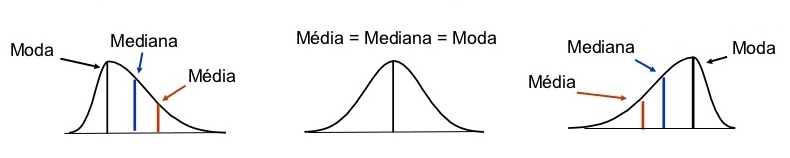
\includegraphics[width=0.9\linewidth]{./img/assimetria} 

}

\caption{Relação medidas descritivas e assimetria}\label{fig:unnamed-chunk-6}
\end{figure}
\end{frame}

\hypertarget{medidas-de-posiuxe7uxe3o-relativa}{%
\section{Medidas de posição
relativa}\label{medidas-de-posiuxe7uxe3o-relativa}}

\begin{frame}{Medidas de posição relativa}
\protect\hypertarget{medidas-de-posiuxe7uxe3o-relativa-1}{}
\beginAHalfColumn

\begin{itemize}
\item
  As medidas de posição relativa ou separatrizes buscam representar
  \textbf{pontos do domínio} em que a variável apresenta porções com
  frequências conhecidas.
\item
  Visam encontrar valores que representam alguma parcela dos dados.
\end{itemize}

\endColumns
\beginAHalfColumn

\begin{itemize}
\tightlist
\item
  Algumas possiblidades são

  \begin{itemize}
  \tightlist
  \item
    Quartis.
  \item
    Decis.
  \item
    Percentis.
  \item
    Máximo.
  \item
    Mínimo.
  \end{itemize}
\end{itemize}

\endColumns
\end{frame}

\begin{frame}{Quartis}
\protect\hypertarget{quartis}{}
\begin{itemize}
\tightlist
\item
  Dividem a amostra em \(4\) partes de mesmo tamanho.
\item
  A ideia para obtenção é similar à da mediana.
\item
  Na verdade, a mediana é um dos quartis: o segundo.
\item
  O primeiro e terceiro quartil são as medianas das duas partes
  divididas pela mediana (método de Tukey).
\end{itemize}
\end{frame}

\begin{frame}{Quartis}
\protect\hypertarget{quartis-1}{}
\begin{itemize}
\tightlist
\item
  O primeiro quartil (\(Q_1\)) é o valor que marca \(1/4\) das
  observações, isto é, \(25\%\).
\item
  O segundo quartil (\(Q_2\)) é o valor que marca \(2/4=1/2\) das
  observações, isto é, \(50\%\) (a mediana).
\item
  O terceiro quartil (\(Q_3\)) é o valor que marca \(3/4\) das
  observações, isto é, \(75\%\).
\item
  A diferença entre primeiro e terceiro quartil é chamada de amplitude
  interquartílica (\(AIQ = Q_3-Q_1\)).
\item
  Estas quantidades são usadas para criação de um poderoso gráfico: o
  boxplot.
\end{itemize}
\end{frame}

\begin{frame}{Quartis}
\protect\hypertarget{quartis-2}{}
\textbf{Exemplo}

\begin{itemize}
\tightlist
\item
  Considere os seguintes valores:
\end{itemize}

\[6; 12; 14;  7; 11;  7;  6; 12;  4; 11;  3;  4;  3;  4;  2\]

\begin{itemize}
\item
  Obtenha os quartis e a amplitude interquartílica.
\item
  Passo 1: ordenar.
\end{itemize}

\begin{longtable}[]{@{}
  >{\raggedright\arraybackslash}p{(\columnwidth - 30\tabcolsep) * \real{0.1356}}
  >{\centering\arraybackslash}p{(\columnwidth - 30\tabcolsep) * \real{0.0508}}
  >{\centering\arraybackslash}p{(\columnwidth - 30\tabcolsep) * \real{0.0508}}
  >{\centering\arraybackslash}p{(\columnwidth - 30\tabcolsep) * \real{0.0508}}
  >{\centering\arraybackslash}p{(\columnwidth - 30\tabcolsep) * \real{0.0508}}
  >{\centering\arraybackslash}p{(\columnwidth - 30\tabcolsep) * \real{0.0508}}
  >{\centering\arraybackslash}p{(\columnwidth - 30\tabcolsep) * \real{0.0508}}
  >{\centering\arraybackslash}p{(\columnwidth - 30\tabcolsep) * \real{0.0508}}
  >{\centering\arraybackslash}p{(\columnwidth - 30\tabcolsep) * \real{0.0508}}
  >{\centering\arraybackslash}p{(\columnwidth - 30\tabcolsep) * \real{0.0508}}
  >{\centering\arraybackslash}p{(\columnwidth - 30\tabcolsep) * \real{0.0678}}
  >{\centering\arraybackslash}p{(\columnwidth - 30\tabcolsep) * \real{0.0678}}
  >{\centering\arraybackslash}p{(\columnwidth - 30\tabcolsep) * \real{0.0678}}
  >{\centering\arraybackslash}p{(\columnwidth - 30\tabcolsep) * \real{0.0678}}
  >{\centering\arraybackslash}p{(\columnwidth - 30\tabcolsep) * \real{0.0678}}
  >{\centering\arraybackslash}p{(\columnwidth - 30\tabcolsep) * \real{0.0678}}@{}}
\caption{Valores ordenados.}\tabularnewline
\toprule()
\endhead
Posição & 1 & 2 & 3 & 4 & 5 & 6 & 7 & 8 & 9 & 10 & 11 & 12 & 13 & 14 &
15 \\
Valor & 2 & 3 & 3 & 4 & 4 & 4 & 6 & 6 & 7 & 7 & 11 & 11 & 12 & 12 &
14 \\
\bottomrule()
\end{longtable}
\end{frame}

\begin{frame}{Quartis}
\protect\hypertarget{quartis-3}{}
\beginAHalfColumn

\textbf{Exemplo}

\begin{itemize}
\tightlist
\item
  Passo 2: obter o segundo quartil (mediana).

  \begin{itemize}
  \tightlist
  \item
    Número de elementos: \(15\).
  \item
    Posição do segundo quartil: \(8\).
  \item
    Valor do segundo quartil: \(6\).
  \end{itemize}
\item
  Passo 3: obter a mediana dos valores da primeira parcela.

  \begin{itemize}
  \tightlist
  \item
    Número de elementos: \(7\).
  \item
    Posição do segundo quartil: \(3\).
  \item
    Valor do segundo quartil: \(4\).
  \end{itemize}
\end{itemize}

\endColumns
\beginAHalfColumn

\begin{itemize}
\item
  Passo 4: obter a mediana dos valores da segunda parcela.

  \begin{itemize}
  \tightlist
  \item
    Número de elementos: \(7\).
  \item
    Posição do segundo quartil: \(3\).
  \item
    Valor do segundo quartil: \(11\).
  \end{itemize}
\item
  \(Q_1 = 4\), \(Q_2 = 6\), \(Q_3 = 11\).
\item
  Amplitude interquartílica.
\end{itemize}

\[AIQ = Q_3 - Q_1 = 11 - 4 = 7\]

\endColumns
\end{frame}

\begin{frame}{Quartis e o Box-plot}
\protect\hypertarget{quartis-e-o-box-plot}{}
\begin{itemize}
\tightlist
\item
  O box-plot faz uso dos quartis para obtenção de um gráfico.
\item
  É possível analisar a distribuição dos dados: posição, variabilidade,
  assimetria, valores atípicos.
\end{itemize}

\begin{figure}

{\centering 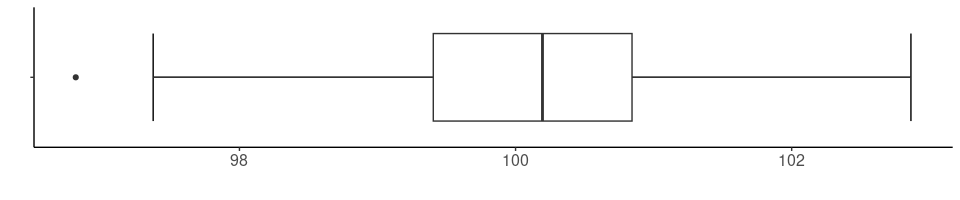
\includegraphics[width=0.9\linewidth]{./img/boxplot0} 

}

\caption{Ilustração box-plot completo.}\label{fig:unnamed-chunk-8}
\end{figure}
\end{frame}

\begin{frame}{Quartis e o Box-plot}
\protect\hypertarget{quartis-e-o-box-plot-1}{}
\begin{itemize}
\tightlist
\item
  A construção de um box-plot inicia-se com um retângulo em que a aresta
  inferior coincide com o primeiro quartil e a superior com o terceiro
  quartil.
\end{itemize}

\begin{figure}

{\centering 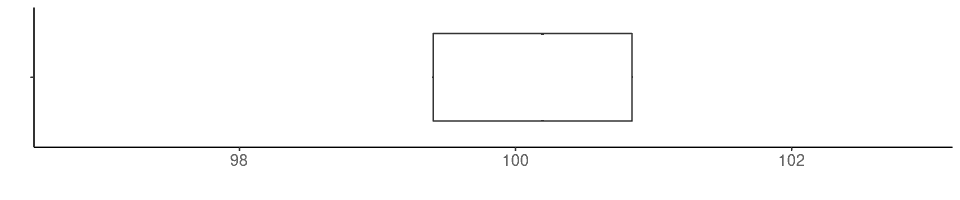
\includegraphics[width=0.9\linewidth]{./img/boxplot1} 

}

\caption{Arestas de um box-plot.}\label{fig:unnamed-chunk-9}
\end{figure}
\end{frame}

\begin{frame}{Quartis e o Box-plot}
\protect\hypertarget{quartis-e-o-box-plot-2}{}
\begin{itemize}
\item
  A mediana é representada por um traço entre as duas arestas.
\item
  De \(Q_1\) até \(Q_3\) estão \(50\%\) das observações centrais, o que
  dá uma ideia a respeito de quão dispersos são os valores.
\end{itemize}

\begin{figure}

{\centering 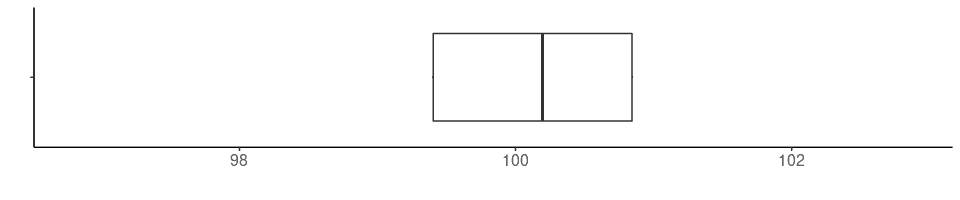
\includegraphics[width=0.9\linewidth]{./img/boxplot2} 

}

\caption{Arestas e mediana emum box-plot.}\label{fig:unnamed-chunk-10}
\end{figure}
\end{frame}

\begin{frame}{Quartis e o Box-plot}
\protect\hypertarget{quartis-e-o-box-plot-3}{}
\begin{itemize}
\item
  Para obtenção da amplitude do box-plot além do retângulo faz-se
  \([Q1-1,5AIQ; Q3+1,5AIQ]\).
\item
  Desenha-se então uma linha até estes valores.
\end{itemize}

\begin{figure}

{\centering 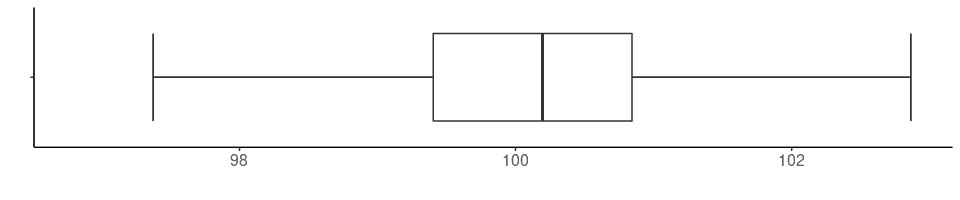
\includegraphics[width=0.9\linewidth]{./img/boxplot3} 

}

\caption{Inclusão dos limites de um box-plot.}\label{fig:unnamed-chunk-11}
\end{figure}
\end{frame}

\begin{frame}{Quartis e o Box-plot}
\protect\hypertarget{quartis-e-o-box-plot-4}{}
\begin{itemize}
\tightlist
\item
  Valores além destes extremos são marcados como um ponto ou asterisco e
  são os candidatos a valores atípicos.
\end{itemize}

\begin{figure}

{\centering 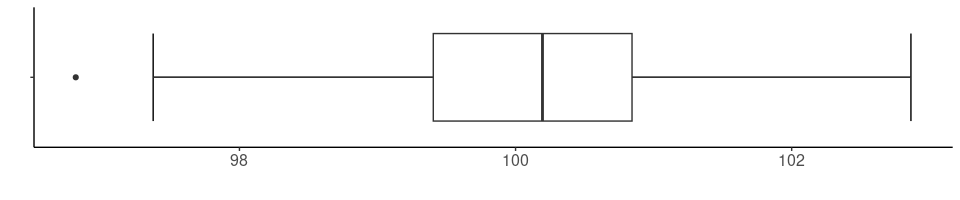
\includegraphics[width=0.9\linewidth]{./img/boxplot0} 

}

\caption{Box-plot completo.}\label{fig:unnamed-chunk-12}
\end{figure}
\end{frame}

\begin{frame}{Outras medidas}
\protect\hypertarget{outras-medidas}{}
\begin{itemize}
\item
  Quartis são a forma mais famosa de particionamento dos dados.
\item
  Porém, qualquer outro percentual pode ser obtido.
\item
  Se temos um conjunto de n valores, organizados de forma crescente, o
  \(P\)-ésimo percentil é um número tal que \(P\%\) dos valores estejam
  à sua esquerda e \((100 - P)\%\) à sua direita.
\item
  Por exemplo, se obtivermos os valores que separam a amostra em \(10\)
  partes com frequência \(1/10\), temos os decis.
\item
  O mínimo e o máximo também são medidas de posição relativa e fornecem
  informação quanto ao domínio da variável.
\end{itemize}
\end{frame}

\hypertarget{medidas-de-dispersuxe3o}{%
\section{Medidas de dispersão}\label{medidas-de-dispersuxe3o}}

\begin{frame}{Medidas de dispersão}
\protect\hypertarget{medidas-de-dispersuxe3o-1}{}
\beginAHalfColumn

\begin{itemize}
\tightlist
\item
  As medidas de dispersão são utilizadas para expressar informações como
  o \textbf{domínio} da variável, grau de \textbf{dispersão} ao redor do
  centro (\textbf{variabilidade}), e também \textbf{distanciamento} dos
  valores com relação ao centro.
\end{itemize}

\endColumns
\beginAHalfColumn

\begin{itemize}
\tightlist
\item
  Algumas medidas possíveis são

  \begin{itemize}
  \tightlist
  \item
    Amplitude.
  \item
    Desvio absluto (médio ou mediano).
  \item
    Variância.
  \item
    Desvio padrão.
  \item
    Coeficiente de variação.
  \end{itemize}
\end{itemize}

\endColumns
\end{frame}

\begin{frame}{Medidas de dispersão}
\protect\hypertarget{medidas-de-dispersuxe3o-2}{}
\begin{itemize}
\item
  Em geral usamos uma medida de posição central, que nos dá uma ideia de
  centro dos dados.
\item
  Mas conjuntos de dados com diferentes valores podem gerar as mesmas
  medidas de posição.
\item
  E mesmo com medidas de posição idêncitas, um pode ser mais disperso
  que o outro.
\item
  Portanto complementamos a informação a respeito do centro com uma
  medida de dispersão, que nos dá uma noção de quão dispersos são os
  dados.
\item
  Outra utilidade das medidas de dispersão é expressar o domínio da
  variável.
\end{itemize}
\end{frame}

\begin{frame}{Amplitude total}
\protect\hypertarget{amplitude-total}{}
\begin{itemize}
\tightlist
\item
  Diferença entre o maior e o menor valor da variável.
\item
  Sensível a valores extremos.
\item
  Usa apenas duas medidas.
\end{itemize}

\[Amp = max(y) - min(y) = y(n) - y(1)\]
\end{frame}

\begin{frame}{Amplitude total}
\protect\hypertarget{amplitude-total-1}{}
\textbf{Exemplo}

\begin{itemize}
\tightlist
\item
  Retomando o problema das notas de 10 alunos, em que as notas obtidas
  foram:
\end{itemize}

\[60;\ 65;\ 77;\ 95;\ 56;\ 94;\ 97;\ 81;\ 80;\ 48\]

\begin{itemize}
\tightlist
\item
  A amplitude é dada pelo maior menos o menor valor:
\end{itemize}

\[Amp = 97 - 58  = 49\]
\end{frame}

\begin{frame}{Desvio absoluto médio}
\protect\hypertarget{desvio-absoluto-muxe9dio}{}
\begin{itemize}
\tightlist
\item
  Um desvio absoluto médio é uma medida de distância da observação para
  uma medida de posição central.
\item
  Podemos usar como referência a média ou a mediana.
\item
  Tomamos todos os desvios absolutos.
\item
  Calculamos a média.
\end{itemize}

\beginAHalfColumn

\[
\text{desvio m\'edio} = \frac{1}{n}
      \sum_{i = 1}^n |(y_i - \overline{y})|
\]

\endColumns
\beginAHalfColumn

\[
\text{desvio mediano} =
      \frac{1}{n} \sum_{i = 1}^n |(y_i - md)|
\]

\endColumns
\end{frame}

\begin{frame}{Desvio}
\protect\hypertarget{desvio}{}
\textbf{Exemplo}

\begin{itemize}
\tightlist
\item
  Retomando o problema das notas de 10 alunos, em que as notas obtidas
  foram:
\end{itemize}

\[60;\ 65;\ 77;\ 95;\ 56;\ 94;\ 97;\ 81;\ 80;\ 48\]

\begin{itemize}
\item
  A média é \(\overline{y} = 75,3\) e a mediana é \(md = 78,5\).
\item
  Obtenha o desvio médio e mediano.
\end{itemize}
\end{frame}

\begin{frame}{Desvio}
\protect\hypertarget{desvio-1}{}
\textbf{Exemplo - desvio médio}

\[
\text{desvio m\'edio} = \frac{1}{10}
       \left ( |(60 - 75,3)| + |(65 - 75,3)| ... + |(80 - 75,3)| + |(48 - 75,3)| \right )
\] \[
\text{desvio m\'edio} = \frac{1}{10}
       \left ( 15,3 + 10,3 ... + 4,7  + 27,3  \right ) = 14,44
\]
\end{frame}

\begin{frame}{Desvio}
\protect\hypertarget{desvio-2}{}
\textbf{Exemplo - desvio mediano}

\[
\text{desvio mediano} = \frac{1}{10}
       \left ( |(60 - 78,5)| + |(65 - 78,5)| ... + |(80 - 78,5)| + |(48 - 78,5)| \right )
\] \[
\text{desvio mediano} = \frac{1}{10}
       \left ( 18,5 + 13,5 ... + 1,5  + 30,5  \right ) = 14,1
\]
\end{frame}

\begin{frame}{Variância e Desvio padrão}
\protect\hypertarget{variuxe2ncia-e-desvio-padruxe3o}{}
\begin{itemize}
\tightlist
\item
  Em vez dos desvios, usa a soma dos quadrados dos desvios em relação à
  média.
\end{itemize}

\[
s^2 = \textrm{Var}(y) = \frac{1}{n - 1} \sum_{i = 1}^{n} (y_i - \overline{y})^2 = \frac{1}{n - 1}\left(\sum_{i = 1}^{n} y_i^2 - \frac{(\sum_{i = 1}^{n} y_i)^2}{n}\right)
\]

\begin{itemize}
\item
  Variância populacional (\(\sigma^2\)): usa apenas \(n\) no demominador
  e é usada quando temos todos os elementos da população. Caso
  contrário, calculamos sempre a estimativa amostral (\(s^2\)).
\item
  Para ter uma medida de dispersão com a mesma unidade de medida dos
  dados originais definiu-se o desvio-padrão como a raiz quadrada da
  variância.
\end{itemize}

\[
s = \sqrt{s^2}
\]
\end{frame}

\begin{frame}{Regra empírica variância e desvio padrão}
\protect\hypertarget{regra-empuxedrica-variuxe2ncia-e-desvio-padruxe3o}{}
Quando a distribuição dos dados é simétrica sabemos que:

\begin{itemize}
\item
  Aproximadamente \(68\%\) das observações estão entre mais ou menos um
  desvio padrão.
\item
  Aproximadamente \(95\%\) das observações estão entre mais ou menos
  dois desvios padrões.
\item
  Aproximadamente \(100\%\) das observações estão entre mais ou menos
  três desvios padrões.
\end{itemize}
\end{frame}

\begin{frame}{Variância e desvio padrão}
\protect\hypertarget{variuxe2ncia-e-desvio-padruxe3o-1}{}
\textbf{Exemplo}

\begin{itemize}
\tightlist
\item
  Retomando o problema das notas de 10 alunos, em que as notas obtidas
  foram:
\end{itemize}

\[60;\ 65;\ 77;\ 95;\ 56;\ 94;\ 97;\ 81;\ 80;\ 48\]

\begin{itemize}
\item
  A média é \(\overline{y} = 75,3\).
\item
  Obtenha o variância e desvio padrão.
\end{itemize}
\end{frame}

\begin{frame}{Variância e desvio padrão}
\protect\hypertarget{variuxe2ncia-e-desvio-padruxe3o-2}{}
\textbf{Exemplo}

\begin{itemize}
\tightlist
\item
  Primeira maneira:
\end{itemize}

\[
s^2 = \textrm{Var}(y) = \frac{1}{10 - 1} \left ( (60 - 75,3)^2 + (65 - 75,3)^2 + ... + (80 - 75,3)^2 + (48 - 75,3)^2   \right )
\]

\[
s^2 = \textrm{Var}(y) = \frac{1}{9} \left ( (-15,3)^2 + (-10,3)^2 + ... + (4,7)^2 + (-27,3)^2   \right )
\]

\[
s^2 = \textrm{Var}(y) = \frac{1}{9} \left ( 234,09 + 106,09 + ... + 22,09 + 745,29 \right ) = 302,68
\]

\[ s = \sqrt{s^2} = \sqrt{302,68} = 17,4\]
\end{frame}

\begin{frame}{Variância e desvio padrão}
\protect\hypertarget{variuxe2ncia-e-desvio-padruxe3o-3}{}
\textbf{Exemplo}

\begin{itemize}
\tightlist
\item
  Segunda maneira:
\end{itemize}

\[
s^2 = \textrm{Var}(y) = \frac{1}{n - 1}\left(\sum_{i = 1}^{n} y_i^2 - \frac{(\sum_{i = 1}^{n} y_i)^2}{n}\right)
\]

\[
s^2 = \textrm{Var}(y) = \frac{1}{9}\left(59425
 - \frac{753^2}{10}\right) = \frac{1}{9}\left(59425
 - 56700.9\right) = 302,68
\]

\[ s = \sqrt{s^2} = \sqrt{302,68} = 17,4\]
\end{frame}

\begin{frame}{Coeficiente de variação}
\protect\hypertarget{coeficiente-de-variauxe7uxe3o}{}
\begin{itemize}
\tightlist
\item
  Medida de variabilidade relativa à média.
\item
  Quociente do desvio-padrão pela média.
\item
  Medida adimensional, geralmente apresentada na forma de porcentagem.
\item
  Permite comparar a variabilidade de variáveis de diferentes naturezas
\end{itemize}

\[
\textrm{CV} = 100 \cdot \frac{s}{\overline{y}}
\]
\end{frame}

\begin{frame}{Coeficiente de variação}
\protect\hypertarget{coeficiente-de-variauxe7uxe3o-1}{}
\textbf{Exemplo}

\begin{itemize}
\tightlist
\item
  Retomando o problema das notas de 10 alunos, em que as notas obtidas
  foram:
\end{itemize}

\[60;\ 65;\ 77;\ 95;\ 56;\ 94;\ 97;\ 81;\ 80;\ 48\]

\begin{itemize}
\item
  A média é \(\overline{y} = 75,3\) e o desvio padrão é \(s = 17,4\).
\item
  Obtenha o coeficiente de variação.
\end{itemize}

\[
\textrm{CV} = 100 \cdot \frac{17,4}{75,3} = 23,11
\]
\end{frame}

\begin{frame}{Desvio, variância, desvio padrão, coeficiente de variação}
\protect\hypertarget{desvio-variuxe2ncia-desvio-padruxe3o-coeficiente-de-variauxe7uxe3o}{}
\begin{itemize}
\item
  A amplitude é simples de calcular, mas é influenciada por valores
  extremos.
\item
  Os desvios absolutos (médio ou mediano) são menos influenciados por
  valores extremos.
\item
  Variância e desvio padrão são influenciados por valores extremos mas
  tem propriedades favoráveis.
\item
  O coeficiente de variação permite comparar a variabilidade de
  variáveis em diferentes escalas.
\item
  Para variáveis qualitativas existem medidas que avaliam a dispersão
  são funções das frequências das classes, como a entropia.
\end{itemize}
\end{frame}

\begin{frame}{}
\protect\hypertarget{section}{}
\beginAHalfColumn

\textbf{O que foi visto:}

\begin{itemize}
\tightlist
\item
  Resumos numéricos.
\item
  Medidas de posição central.
\item
  Medidas de posição relativa.
\item
  Medidas de dispersão.
\end{itemize}

\endColumns
\beginAHalfColumn

\textbf{Próximos assuntos:}

\begin{itemize}
\tightlist
\item
  Análises bivariadas.

  \begin{itemize}
  \tightlist
  \item
    Qualitativa x qualitativa.
  \item
    Quantitativa x quantitativa.
  \item
    Quantitativa x qualitativa.
  \end{itemize}
\end{itemize}

\endColumns
\end{frame}

\end{document}
